% Select language used in document (ngerman or english). Automatically
% generated text is translated accordingly.
% use \selectthesislanguage in body.tex to switch to default language

\documentclass[english, paper]{mmt} % use for BA1
%\documentclass[ngerman, bachelorthesis]{mmt} % use for BA2
%\documentclass[ngerman, masterthesis]{mmt} % use for Master thesis

\usepackage{mathptmx}
\usepackage{graphicx}
\usepackage{times}
\usepackage{subfig}
\usepackage{float}
\usepackage[utf8]{inputenc}
\usepackage{listings}
\usepackage{makecell}
\usepackage[toc,page]{appendix}
\usepackage{hyperref}
\hypersetup{
    colorlinks,
    citecolor=black,
    filecolor=black,
    linkcolor=black,
    urlcolor=black
}
\usepackage{breakurl}

\usepackage{amsmath}
\usepackage[autostyle,german=guillemets]{csquotes}

% moved to cls file. use \selectthesislanguage to switch to default language
%\usepackage[english,ngerman]{babel}

\usepackage{abbrevs}
%% the following solves a bug in the abbrevs package, that adds an empty
%% space after the abbrev
\makeatletter
\renewcommand\maybe@space@{%
  % \@tempswatrue % <= this is in the original
  \maybe@ictrue % <= this is new
  \expandafter   \@tfor
    \expandafter \reserved@a
    \expandafter :%
    \expandafter =%
                 \nospacelist
                 \do \t@st@ic
  % \if@tempswa % <= this is in the original
  \ifmaybe@ic % <= this is new
    \space
  \fi
}
\makeatother
%%


\usepackage{listings}
\usepackage{color}
\definecolor{lightgray}{rgb}{.9,.9,.9}
\definecolor{darkgray}{rgb}{.4,.4,.4}
\definecolor{purple}{rgb}{0.65, 0.12, 0.82}
\lstdefinelanguage{JavaScript}{
  keywords={break, case, catch, continue, debugger, default, delete, do, else, false, finally, for, function, if, in, instanceof, new, null, return, switch, this, throw, true, try, typeof, var, let, const, void, while, with},
  morecomment=[l]{//},
  morecomment=[s]{/*}{*/},
  morestring=[b]',
  morestring=[b]",
  ndkeywords={class, export, boolean, throw, implements, import, this},
  keywordstyle=\color{blue}\bfseries,
  ndkeywordstyle=\color{darkgray}\bfseries,
  identifierstyle=\color{black},
  commentstyle=\color{purple}\ttfamily,
  stringstyle=\color{red}\ttfamily,
  sensitive=true
}

\lstset{
   language=JavaScript,
   backgroundcolor=\color{lightgray},
   extendedchars=true,
   basicstyle=\footnotesize\ttfamily,
   showstringspaces=false,
   showspaces=false,
   numbers=left,
   numberstyle=\footnotesize,
   numbersep=9pt,
   tabsize=2,
   breaklines=true,
   showtabs=false,
   captionpos=b
}

\usepackage[authordate,bibencoding=auto,strict,noibid,backend=biber]{biblatex-chicago}
\bibliography{bibliography}

%% Add configuration options
\newabbrev{\authorname}{Natasha Troth}
\newabbrev{\authormail}{ntroth.mmt-b2017@fh-salzburg.ac.at}
\newabbrev{\titlename}{Understanding, Detecting and Preventing Bots in Online Social Networks}
\newabbrev{\advisor}{FH-Prof. DI Dr. Simon Ginzinger, MSc}
%\newabbrev{\secondadvisor}{Titel Vorname Nachname}
\newabbrev{\thesisdate}{23.04.2019}
\newabbrev{\keywordsenglish}{Bots, Online Social Networks, Exploitation}
\newabbrev{\keywordsgerman}{wort1, wort2, wort3}


%% Paper title.

\title{\titlename}

%% This is how authors are specified in the conference style

%% Author 
\author{ \authorname\\ \scriptsize \authormail \\ \scriptsize 
\ifmmtlanguagegerman FH Salzburg \else Salzburg University of Applied Sciences \fi
}

%% A teaser figure can be included as follows, but is not recommended since
%% the space is now taken up by a full width abstract.
%\teaser{
%  \includegraphics[width=1.5in]{sample.eps}
%  \caption{This can be a teaser image of the thesis.}
%}

%% Abstract section for paper format.
\abstract{
    \ifmmtlanguagegerman 
        \selectlanguage{ngerman}
        Bots sind Programme, die verschiedene Aufgaben automatisieren können. Angreifer können Bots missbrauchen, um Konten in Online Sozialen Netzwerken (OSN) zu kontrollieren und um die Meinungen der Benutzer möglicherweise zu beeinflussen. Dies machen sie indem sie falsche Informationen und Propaganda verbreiten. Solche Bots könnten beispielsweise von Politikern verwendet werden, um die Unterstützung eines politischen Kandidaten zu steigern.
Diese Bachelorarbeit erklärt was Bots sind, wie sie auf OSNs missbraucht werden können, welche Schwachstellen OSNs aufweisen und was man tun kann, um Bots zu erkennen. Einige Bots werden erstellt, um für Menschen hilfreich zu sein. Andere können von Angreifern missbraucht werden, um ein scheinbar realistisches OSN-Konto zu erstellen. Damit können sie sich mit anderen Benutzern verbinden und Informationen mit ihnen teilen (durch Re-posting oder Erstellen synthetischer Nachrichten). Um Bot-Infiltrationen zu verhindern, müssen aktuelle Schwachstellen in OSNs behoben werden. Beispiele für solche Schwachstellen sind die Verwendung ineffektiver CAPTCHAs, die Verwendung von Sybil-Konten und gefälschten Profilen, durchforstbare Social Graphs und ausnutzbare Plattformen und APIs. Da die OSN Sicherheitsvorkehrungen bei der Erkennung von Bot-Infiltrationen vorteilhafter sind, anstatt diese zu verhindern, konzentriert sich diese Arbeit mehr auf die Erkennung von Bots.
Das Ziel eines Angreifers besteht in der Regel darin, Socialbots zu verwenden, um eine Vielzahl von Benutzern zu beeinflussen und Inhalte mit ihnen zu teilen. Dabei weisen diese Bots bestimmte Verhaltensweisen auf, die zur Erkennung dieser verwendet werden können. Dazu gehört beispielsweise übermäßig automatisch erstellter Inhalt, das Benutzen von böswilliger URLs, aggressives Following-Verhalten oder lange Online-Sitzungen. Daraufhin werden in diesem Artikel die Ergebnisse der \glqq DARPA Twitter Bot Detection Challenge\grqq{} und eine beliebte Plattform \glqq Botometer\grqq{}{} (ehemals \glqq BotOrNot\grqq{}) vorgestellt, die mithilfe der Feature-Based Erkennung Twitter Konten als Bot oder kein Bot zu klassifizieren. Weitere Erkennungssysteme werden angeschaut, wie die \glqq Associative Affinity Factor Analysis\grqq{} (AAFA), die eine Genauigkeit von 0,96 erreichte, während BotOrNot nur 0,66 erreichte.

    \else 
        \selectlanguage{english}
        Bots are programmes that can automate a number of diverse tasks. Adversaries can misuse bots to control accounts on Online Social Networks (OSNs) and potentially sway peoples' opinions by spreading misinformation and propaganda. These bots can for example be used by politicians to inflate the level of support for a political candidate.
This bachelor thesis explains what bots are, how they can be misused in OSNs, what vulnerabilities OSNs exhibit and what can be done to detect bots. Some bots are created to be helpful to humans. Other bots can be misused by adversaries to create a seemingly realistic OSN account. The account can then be utilised to connect with other users and share information with them (through re-posting or creating synthetic messages). In order to prevent bot infiltrations, current weaknesses in OSNs would need to be fixed. Examples given for these are the use of ineffective CAPTCHAs, the use of Sybil accounts and fake profiles, crawlable social graphs, and exploitable platforms and APIs. Since OSN security defences are more advantageous in detecting bot infiltrations, rather than preventing them, this thesis focuses more on detecting bots. 
An adversary's goal typically is to use socialbots to influence a wide range of users and share content with them. In doing so, these bots exhibit certain behavioural patterns, which can be exploited to detect them. Examples for such patterns include excessive automatically created content, presence of malicious URLs, aggressive following behaviour, or long online sessions. This paper further reviews the results of the "DARPA Twitter Bot Detection Challenge” and the industry's goto platform “Botometer” (formerly "BotOrNot"), which use feature-based detection to classify Twitter accounts as bots or not bots. Other detection systems are examined, such as the "Associative Affinity Factor Analysis" (AAFA), which achieved 0.96 accuracy, while BotOrNot only achieved 0.66.

    \fi
}

%%%%%%%%%%%%%%%%%%%%%%%%%%%%%%%%%%%%%%%%%%%%%%%%%%%%%%%%%%%%%%%%
%%%%%%%%%%%%%%%%%%%%%% START OF THE PAPER %%%%%%%%%%%%%%%%%%%%%%
%%%%%%%%%%%%%%%%%%%%%%%%%%%%%%%%%%%%%%%%%%%%%%%%%%%%%%%%%%%%%%%%%

\begin{document}
% TODO switch for english, german
\selectthesislanguage

\pagenumbering{gobble}

 % group open
\ifmmtpaper 
\begingroup 
    % is required because paper template messes with sizes
    \fontsize{12}{18}\selectfont        
    \setlength{\parindent}{0pt}
    \setlength{\parskip}{5pt plus 2pt minus 1pt}
    \sectionfont{\fontsize{14}{15}\selectfont}
\fi

    \begin{titlepage}

% check if second advisor exists
\newcommand{\printsecondadvisor}[1]{%
  \ifcsname#1\endcsname%
  \ifmmtlanguagegerman ZweitbetreuerIn: \else Second Advisor: \fi \secondadvisor 
  \else%
    
  \fi%
}

\ifmmtmasterthesis

    
    % \begin{center}
    %     \Huge{ 
    %     	\textbf{\ifmmtlanguagegerman Masterarbeit \else Master Thesis \fi}
    %     }
    % \end{center}
    
    \newpage
    
    \thispagestyle{empty}
    
    \hfill 
\includegraphics[height=1.5cm]{images/FHSLogo.jpg}
    
    \vspace*{2cm}
    
    \Large{
    \titlename
    
    \vspace*{1cm}
    
    \ifmmtlanguagegerman
    Masterarbeit zur Erlangung des akademischen Grades
    \else
    Master thesis in partial fulfilment of the requirements for\\ the degree of 
    \fi
    
    \vspace*{0.5cm}
    
    \textit{Master of Science}
    }
    
    
    \vspace*{1.5cm}
    {\large
    \ifmmtlanguagegerman AutorIn: \else Author: \fi \authorname
    }
    \vfill
    
    {\normalsize
    \ifmmtlanguagegerman
    Vorgelegt am FH-Masterstudiengang MultiMediaTechnology, Fachhochschule Salzburg
    \else
    Submitted to the Master degree program MultiMediaTechnology, Salzburg University of Applied Sciences
    \fi
    
    
    \vspace*{1cm}
    
    \ifmmtlanguagegerman BetreuerIn: \else Advisor: \fi
    \advisor
    \\    
    \printsecondadvisor{secondadvisor}
    
    \vfill
    
    Salzburg, \ifmmtlanguagegerman Österreich, \else Austria, \fi  \thesisdate
    }

\else % Bachelor thesis title page

    \begin{center}
    
    
\includegraphics[width=5cm]{images/FHSLogo.jpg}


    \vspace*{4cm}
    
    \fontsize{20.79}{18pt}{\selectfont        
    %\Large{
    	\textit{\textbf{\titlename}}
    %}
    }
    
    \vspace*{4cm}
    
    \fontsize{20.79}{18pt}{%\large{
    \ifmmtlanguagegerman
    	\textbf{Bachelorarbeit \ifmmtpaper 1 \else 2 \fi }
    \else
        \textbf{Bachelor Thesis \ifmmtpaper 1 \else 2 \fi }
    \fi
    }
    
    
    \end{center}
    
    \vfill
    
    %\begin{tabular}{ll}
    \ifmmtlanguagegerman AutorIn: \else Author: \fi  \authorname  \\
    \ifmmtlanguagegerman BetreuerIn: \else Advisor: \fi \advisor \\
    \printsecondadvisor{secondadvisor}
    
    Salzburg, \ifmmtlanguagegerman Österreich, \else Austria, \fi \thesisdate
    
    
    
    % uncomment the following 3 lines for an optional lock flag, max. 2 years!
    %\hfill
    %\color{red}
    %\framebox{Sperrvermerk bis 20/01/2012}

\fi

\end{titlepage}
        
    \onecolumn           
    
    \pagenumbering{roman}
    
    \newpage
    
\ifmmtlanguagegerman
\subsection*{Eidesstattliche Erklärung}


Ich erkläre hiermit eidesstattlich, dass  ich  die vorliegende Arbeit selbständig  und ohne fremde Hilfe verfasst, und keine  anderen  als die angegeben Quellen und  Hilfsmittel benutzt  habe. Weiter versichere ich hiermit, dass ich   die den benutzten Quellen  wörtlich oder inhaltlich entnommenen Stellen als solche kenntlich gemacht habe.

Die Arbeit wurde bisher in gleicher oder ähnlicher Form keiner anderen Prüfungskommission weder im In- noch im Ausland vorgelegt und auch nicht veröffentlicht.

\else

\subsection*{Affidavit}

I herewith declare on oath that I wrote the present thesis without the help of third persons and without using any other sources and means listed herein; I further declare that I observed the guidelines for scientific work in the quotation of all unprinted sources, printed literature and phrases and concepts taken either word for word or according to meaning from the Internet and that I referenced all sources accordingly.

This thesis has not been submitted as an exam paper of identical or similar form, either in Austria or abroad and corresponds to the paper graded by the assessors.

\fi

\vspace*{3cm}

%{\bf \thesisdate{}}


\hfill

\ifmmtlanguagegerman
$\overline{Datum \hspace{2cm}}$ \hfill $\overline{{Unterschrift}\hspace{3cm}}$

\vspace*{1cm}

\hfill $\overline{{Vorname\hspace{2cm}Nachname}}$
 
 \else
 $\overline{Date \hspace{2cm}}$ \hfill $\overline{{Signature}\hspace{4cm}}$

\vspace*{1cm}

 \hfill $\overline{{First~Name\hspace{2cm}Last~Name}}$
 \fi

  % comment out for expose

% group closing
\ifmmtpaper
\endgroup
\fi

%\ifmmtpaper\else
    
    \newpage
    \selectlanguage{ngerman}
    \section*{Kurzfassung}
    Bots sind Programme, die verschiedene Aufgaben automatisieren können. Angreifer können Bots missbrauchen, um Konten in Online Sozialen Netzwerken (OSN) zu kontrollieren und um die Meinungen der Benutzer möglicherweise zu beeinflussen. Dies machen sie indem sie falsche Informationen und Propaganda verbreiten. Solche Bots könnten beispielsweise von Politikern verwendet werden, um die Unterstützung eines politischen Kandidaten zu steigern.
Diese Bachelorarbeit erklärt was Bots sind, wie sie auf OSNs missbraucht werden können, welche Schwachstellen OSNs aufweisen und was man tun kann, um Bots zu erkennen. Einige Bots werden erstellt, um für Menschen hilfreich zu sein. Andere können von Angreifern missbraucht werden, um ein scheinbar realistisches OSN-Konto zu erstellen. Damit können sie sich mit anderen Benutzern verbinden und Informationen mit ihnen teilen (durch Re-posting oder Erstellen synthetischer Nachrichten). Um Bot-Infiltrationen zu verhindern, müssen aktuelle Schwachstellen in OSNs behoben werden. Beispiele für solche Schwachstellen sind die Verwendung ineffektiver CAPTCHAs, die Verwendung von Sybil-Konten und gefälschten Profilen, durchforstbare Social Graphs und ausnutzbare Plattformen und APIs. Da die OSN Sicherheitsvorkehrungen bei der Erkennung von Bot-Infiltrationen vorteilhafter sind, anstatt diese zu verhindern, konzentriert sich diese Arbeit mehr auf die Erkennung von Bots.
Das Ziel eines Angreifers besteht in der Regel darin, Socialbots zu verwenden, um eine Vielzahl von Benutzern zu beeinflussen und Inhalte mit ihnen zu teilen. Dabei weisen diese Bots bestimmte Verhaltensweisen auf, die zur Erkennung dieser verwendet werden können. Dazu gehört beispielsweise übermäßig automatisch erstellter Inhalt, das Benutzen von böswilliger URLs, aggressives Following-Verhalten oder lange Online-Sitzungen. Daraufhin werden in diesem Artikel die Ergebnisse der \glqq DARPA Twitter Bot Detection Challenge\grqq{} und eine beliebte Plattform \glqq Botometer\grqq{}{} (ehemals \glqq BotOrNot\grqq{}) vorgestellt, die mithilfe der Feature-Based Erkennung Twitter Konten als Bot oder kein Bot zu klassifizieren. Weitere Erkennungssysteme werden angeschaut, wie die \glqq Associative Affinity Factor Analysis\grqq{} (AAFA), die eine Genauigkeit von 0,96 erreichte, während BotOrNot nur 0,66 erreichte.

    \ifmmtmasterthesis
    
    \vspace*{0.5cm} 
    \textbf{Schlüsselwörter:~} \keywordsgerman
    \fi
    \newpage
    \selectlanguage{english}
    \section*{Abstract}
    Bots are programmes that can automate a number of diverse tasks. Adversaries can misuse bots to control accounts on Online Social Networks (OSNs) and potentially sway peoples' opinions by spreading misinformation and propaganda. These bots can for example be used by politicians to inflate the level of support for a political candidate.
This bachelor thesis explains what bots are, how they can be misused in OSNs, what vulnerabilities OSNs exhibit and what can be done to detect bots. Some bots are created to be helpful to humans. Other bots can be misused by adversaries to create a seemingly realistic OSN account. The account can then be utilised to connect with other users and share information with them (through re-posting or creating synthetic messages). In order to prevent bot infiltrations, current weaknesses in OSNs would need to be fixed. Examples given for these are the use of ineffective CAPTCHAs, the use of Sybil accounts and fake profiles, crawlable social graphs, and exploitable platforms and APIs. Since OSN security defences are more advantageous in detecting bot infiltrations, rather than preventing them, this thesis focuses more on detecting bots. 
An adversary's goal typically is to use socialbots to influence a wide range of users and share content with them. In doing so, these bots exhibit certain behavioural patterns, which can be exploited to detect them. Examples for such patterns include excessive automatically created content, presence of malicious URLs, aggressive following behaviour, or long online sessions. This paper further reviews the results of the "DARPA Twitter Bot Detection Challenge” and the industry's goto platform “Botometer” (formerly "BotOrNot"), which use feature-based detection to classify Twitter accounts as bots or not bots. Other detection systems are examined, such as the "Associative Affinity Factor Analysis" (AAFA), which achieved 0.96 accuracy, while BotOrNot only achieved 0.66.

    \ifmmtmasterthesis
        
    \vspace*{0.5cm} 
    \textbf{Keywords:~} \keywordsenglish
    \fi
    \selectthesislanguage
    
    \newpage
    \tableofcontents
    
    \newpage
    \listoffigures
    %\lstlistoflistings
    %\listoftables
    \ifmmtlanguagegerman
\section*{Abkürzungsverzeichnis}
\else
\section*{Abbreviations}
\fi

\begin{table}[h]		
	\begin{tabular}{ll}
		OSN & Online Social Network \\
		SbN & Socialbot Network \\
		C\&C & Command \& Control \\
		DARPA & Defense Advanced Research Projects Agency \\
		AAFA & Associative Affinity Factor Analysis \\	
		
	\end{tabular}
\end{table}

    
    
%\fi

\mmtcolumnmode % switch back to column formatting of stylesheet

\maketitle % used for paper formatting

\ifmmtpaper\else
\pagestyle{headings}
\fi
\pagenumbering{arabic}


%for reference to this section
\section{Introduction}
\label{section:Introduction}
The word "bot" is an abbreviation for "software robot" \autocite[96]{RiseOfSocialBots}.
\textcite[18-19]{SoftwareBots} clarify, that "bot" typically refers to a conversational-style user interface, an anthropomorphised script or an agent that automates routine and dull responsibilities. They can take on a diverse number of tasks and roles. While many of these functions can be useful, others may be harmful.

\textcite[93]{SocialbotNetwork} explained that "socialbots" are a type of bot that are able to control accounts on Online Social Networks (OSNs). They can be used to post messages, send connection requests and perform other basic tasks on these platforms. Socialbots distinguish themselves from other malicious bot types, as they are designed to be stealthy. By infiltrating OSN users, adversaries can use bots to reach a manipulative position and potentially sway peoples' opinions by spreading misinformation and propaganda. \textcite[98]{RiseOfSocialBots} gave as an example, that bots may be utilised to boost the level of support for a political candidate. By influencing the elections, these bots could be endangering democracy. \textcite[559]{DesignAnalysis} observed, that to productively be able to oppose these foes, one must prevent the factors which enable the bots to infiltrate, namely vulnerabilities found in OSNs. \textcite[2]{AidingDetectionFakeAccounts} pointed out, that attackers are constantly capable of adjusting their behaviour to evade detection, which makes finding a suitable detection software more problematic. \textcite[100]{RiseOfSocialBots} stated, that the advances in this direction are just beginning. The currently employed strategies therefore are not as competent as would be liked. The computing community is currently designing advanced methods to detect socialbots automatically. 

The aim of this bachelor thesis is to explain what bots are, how they operate and what can be done to detect and prevent them from potentially adversely affecting OSN users. Section \ref{section:WhatBotsAre} concentrates on clarifying what bots are, how they operate, how they can be misused and what weaknesses in OSNs can be exploited. Section \ref{section:Detect} focuses on what weaknesses bots display and which methods detection systems use to detect them. The conclusion summarises the findings in this paper. 



\section{What bots are and how they operate on Online Social Networks}
\label{section:WhatBotsAre}
    
    \subsection{Definition and functionality of bots}
    \label{subsection:DefinintionAndFunctionalityBots}
        When computer programmes were first created, people envisioned these to behave like humans. They hoped that these programmes would, for example, automate tasks performed by humans and also collaborate with humans to complete intellectual tasks. People hoped for them to pass the Turing test \autocite[18]{SoftwareBots}. \textcite[25]{turing2009} defined that the Turing test is a test, to see if humans can tell the difference between a human and a computer. According to \textcite[18]{SoftwareBots}, bots have passed this test. 
        
        As introduced before in section \ref{section:Introduction}, \textcite[18]{SoftwareBots} described, that the word “bot” typically refers to a conversational-style user interface, an anthropomorphised script or an agent that automates routine and dull responsibilities. They are often found on platforms where users interact with other users. Bots can take on a diverse number of tasks and roles, such as retrieving, sharing, extracting and analysing data. Furthermore, on social media, bots can detect and monitor events and activities. They can also give feedback and recommendations on tasks.
    
        \subsubsection{Characterisations of bots}
            According to \textcite[19]{SoftwareBots}, bots have taken on diverse tasks and roles, even though their development and spread has only happened in a few years. The authors introduce three ways to characterise bots:
            
            \begin{itemize}
            	\item \textit{Through their interaction model}: Some bots are communicated with via specific commands, while others are able to parse natural language through text or speech. Moreover, there are bots that are activated by a pull-based approach (user initiates interaction, e.g. “Hey Siri”) and there are others that facilitate a push-based approach (bot initiates interaction).
        		\item \textit{Through their intelligence}: Some bots understand their context and change their interaction depending on it (Adaptation). Some adhere to simple logic rules while others utilise artificial intelligence (Reasoning). Finally, some bots need human input while others act autonomously (Autonomy).
        		\item \textit{According to their purpose}: Generalist bots can execute multiple simple tasks and provide the user with external resources when unable to provide accurate knowledge. Examples include Siri and Cortana. Transactional bots automatically execute transactions for users. For example: Making a purchase automatically when the price has reached a certain level. Informational bots provide users with information. For example: Stock insights or weather updates.
            \end{itemize}
            
              \textcite[96]{RiseOfSocialBots} stated that some bots are created to be helpful to humans. 
        An example of useful bots are ones used by Wikipedia, as mentioned by \textcite[79-80]{Wikipedia}. Wikipedia started to grow exponentially in 2004, with the growth peaking in 2007 with more than 180 edits per minute. It became impossible for humans to keep up with reviewing the volume of all the incoming edits. Wikipedia therefore uses bots to automatically handle repetitive tasks, such as monitoring and curating Wikipedia content (e.g. spell checking, spell fixing, and correcting ISBNs), and also protecting the encyclopedia from harmful activity (e.g. reverting vandalism, and reverting content with links to blacklisted domains).
        
        \textcite[98]{RiseOfSocialBots} explains further, that other bots are created to mislead, exploit, and manipulate users’ communication on social media. 
        
        This paper concentrates on the malicious bots that operate on Online Social Networks.
    
    \subsection{Misuse of bots}
    \label{subsection:MisuseOfBots}
      

        \textcite[93]{SocialbotNetwork} described that a "socialbot" is an automation software, that can control an OSN account and is able  perform basic tasks on OSNs (such as Twitter\footnote{https://twitter.com} or Facebook\footnote{https://www.facebook.com}). Under the control of adversary-owned or hijacked accounts, bots can post messages and send connection requests. What distinguishes socialbots from other bots, is that they are designed to act like humans.
        

        According to \textcite[2]{ReverseEngineeringSocialbot}, socialbots are programmed to first gain influence and trust on the targeted OSN. They then conduct malicious activities on that OSN, such as spread misinformation and influence public opinion.
        
        \textcite[556-557, 560]{DesignAnalysis} conducted a study to evaluate the vulnerability of OSNs to large-scale infiltration and how their defence stands against socialbots. In this study, Boshmaf et al. created a Socialbot Network (SbN) and operated it on Facebook for eight weeks. This consisted of 102 programmable socialbots and one software controller (botmaster). These socialbots were maintained by the adversary (botherder), who they belonged to. The three components of the SbN were socialbots, a botmaster and a Command \& Control (C\&C) channel, visualised in figure \ref{figure:socialbotnet}. The bots had the ability to perform operations related to social interactions, such as posting a message, or operations related to the social structure, such as sending a connection request.  As an example of how to build a synthetic message, \textcite[4]{ReverseEngineeringSocialbot} used a Markov generator. As stated by \textcite[116]{Markov}, a Markov process is a random process that can be used to generate different word sequences using a random walk procedure. \textcite[4]{ReverseEngineeringSocialbot} used a set of tweets posted by their target users as a sample set of documents for their Markov generator, in order to increase the consideration of relevance for their messages. 
        
        According to \textcite[560]{DesignAnalysis}, the way the SbN can perform the previously mentioned operations, is by enabling each socialbot to control its own OSN profile and execute commands that result in said operations. These commands can be locally predefined or sent to the bot by the botmaster. Botcargo is the name for any data collected by the socialbots. The socialbots transfer the botcargo to the botmaster via the C\&C channel.
        
        
        \begin{figure*}[h]
        	\centering
        	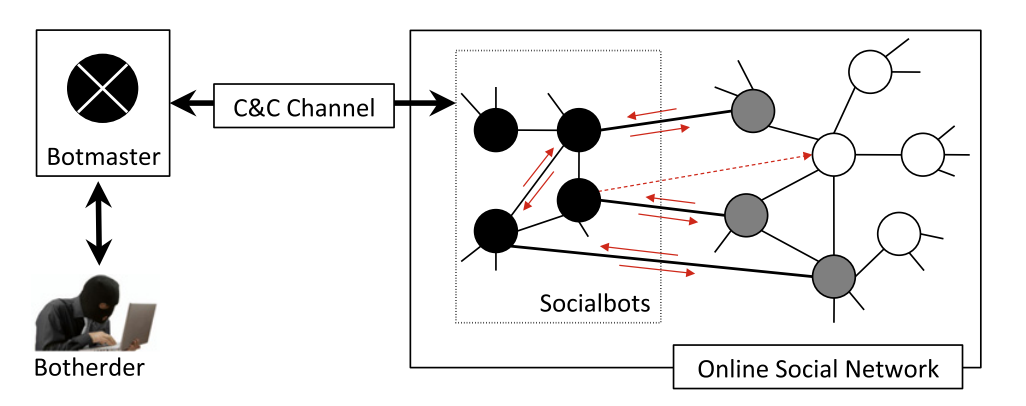
\includegraphics[width=0.9\textwidth]{template-thesis-latex-master/images/SocialbotNetwork.png}
        	\caption{This is the way \textcite[561]{DesignAnalysis} designed their Socialbot Network. Every circle (node) serves as a user profile. The black nodes are socialbots, the grey ones are infiltrated users. The lines connecting two nodes represent connection requests. The red arrows stand for social interactions. 
        	}
        	\label{figure:socialbotnet}
        	
        \end{figure*}
        
         
         From the adversary’s point of view, \textcite[1, 3-5]{DetectingSpammers} tried to understand how spammers on OSNs operate. In order to do so, they created a total of 900 profiles on three (at that time) major OSNs (Facebook, Twitter and MySpace\footnote{https://myspace.com}) and analysed the behaviour of users who contacted those profiles. These accounts acted in a passive way, meaning they only accepted received connection requests and didn’t send any themselves (since the first thing a spammer would most likely do, is send a connection request to get in touch with his or her victims). The study, which ran for a year, showed, that the majority of the received connection requests came from real users who wanted to inflate their popularity on the OSN or were searching for real people with the same name as on the bot's profile, rather than from spam bots. The profiles that were identified as spam bots showed different activity levels and spam delivery strategies.  Stringhini, Kruegel, and Vigna therefore distinguished four different categories of bots:
          \begin{itemize}
        	\item \textit{Displayer}: A bot that displays spam content on its own profile but doesn’t post malicious content. A victim would therefore have to visit the bot’s profile to perceive spam content. This method is presumably the least effective one.
        	\item \textit{Bragger}: These bots post content on their own feed. This results in the spam messages being shown on the connected victims feed. The victim is however the only person who sees this, which means that only people connected to the bot’s profile see the malicious content.
        	\item \textit{Poster}: These bots distribute messages that can be seen not only by connected users, but also by the friends who visit their profile. They do this by posting direct messages to the victim (e.g. on the victims Facebook wall). According to Stringhini, Kruegel, and Vigna, this way of spamming reaches a greater number of users, which makes it the most effective.
        	\item \textit{Whisperer}: These bots send private messages to their connected users who are the only ones who then see them. These messages must be addressed to a specific user.
        \end{itemize}
    
    
    \subsection{Weaknesses in OSNs and consequences}
    \label{subsection:WeaknessesOSNs}
        \textcite[556-559, 573]{DesignAnalysis} explain in their paper, that OSNs are centralised web platforms, on which users own accounts are represented by profiles. Personal data, such as name, gender, interests and contact information are stored in this profile and represent the user’s social attributes. Users can establish social relationships with other users, such as friendships in Facebook or followerships in Twitter. As stated, these platforms can be exploited by adversaries to perform malicious activities. Depending on the user profile privacy settings, such an infiltration can result in a severe privacy breach, where private user data is exposed. The authors discuss that OSN security defences are more advantageous in detecting bot infiltrations, as opposed to preventing them. The authors clarify, that guarding an OSN from bots can be devided into prevention and limitation. Prevention means eliminating factors in the OSN that permit an SbN from operating on it in the first place, whereas with limitation, it is implied that the OSN's operator accepts that infiltrations can happen, and uses methods to limit the ramifications of the infiltration. Since preventing large-scale infiltration would mean fixing inherent vulnerabilities found on OSNs, this would mean solving problems that relate to web automation, online-offline identity binding, and usable security. Four vulnerabilities acknowledged by Boshmaf et al. include the use of ineffective CAPTCHAs, the use of Sybil accounts and fake profiles, crawlable social graphs, and exploitable platforms and APIs. 
        
        \subsubsection{The use of ineffective CAPTCHAs}
            \textcite[559]{DesignAnalysis} explained, that to be able to create a user account on an OSN, the user has to frequently solve a CAPTCHA. CAPTCHAS are employed by OSNs to prevent automated bots from corrupting their system. The reason this is a vulnerability on OSNs, is because adversaries have found multiple techniques to solve these tests when creating malicious accounts. 
            
            \textcite[435, 437, 439]{Captcha} revealed, that a robust ecosystem has been created to solve CAPTCHAs. One approach of solving these is by using Automated Software Solvers, which use basic optical character recognition (OCR) to extract symbols from the distorted CAPTCHA images. Another one is by using Human Solver Services. Since CAPTCHAs are designed to resist automated solvers, human beings should be able to solve them with high probability. Human Solver Services therefore outsource the task of solving them to human labour.
        
        \subsubsection{The use of Sybil accounts and fake profiles}
            \textcite[1]{sybilAttack} defines that a “Sybil\footnote{Schreiber, Flora Rheta. 1973. \textit{Sybil}. New York, N.Y: Warner Books} attack” is when a single entity controls multiple identities. \textcite[558-560]{DesignAnalysis} defines in this context, that an instance of Sybil attack in OSNs is a large-scale infiltration, where adversaries use automated software to control numerous accounts to connect with many users on said OSN. These accounts can be adversary-owned or hijacked accounts (i.e., Sybils). As a consequence of the vulnerabilities on OSNs, attackers are able to automate the full process of creating accounts and can use that to create a series of Sybil accounts. In order to create a new user account, or in this case a new Sybil account, there are two hurdles the adversary must overcome: providing a valid email address and account validation through that address. Adversaries can overcome these hurdles by owning multiple email addresses and by writing a simple script to send a HTTP request to the activation link provided in the activation email. The next step in creating a Sybil account is to create a user profile. This requires the user to provide information about their social attributes. "Socially attractive” profiles have been shown to be more effective in attracting other users’ attention. By crawling the web and finding websites with publicly available pictures and corresponding demographic data, adversaries can extract this information and therefore automate the process of collecting and populating their fake user profiles.
        
        \subsubsection{Crawlable social graphs}
            According to \textcite[560]{DesignAnalysis}, in order to protect users’ privacy, the social graph (i.e., the social structures) of the OSN is normally hidden from public access. However, adversaries have the ability to reconstruct parts of these using web crawling techniques and online search algorithms.
        
        \subsubsection{Exploitable platforms and APIs}
            OSNs offer software APIs so that third-party software systems can integrate the OSNs platform into their systems. Adversaries are able to automate the execution of social activities online by using such APIs \autocite[560]{DesignAnalysis}.

       \bigskip
        A question raised by \textcite[818]{DetectingAutomation} is whether Twitter users are aware of privacy and identity protection settings on said platform. Discoveries revealed that only 4.9\% of Chu et al.'s inspected users had their account set to protected (homepage is only visible to the user’s friends). Twitter’s default setting is to have the accounts set to unprotected.
    

\section{Detect bots in Online Social Networks}
\label{section:Detect}
    \subsection{Behavioural patterns bots display}
    \label{subsection:BehaviouralPatternsBotsDisplay}
    
       In order to understand infiltration strategies into OSNs using socialbots and to which extent bots are able to infiltrate OSNs, \textcite[1-4, 6-9]{ReverseEngineeringSocialbot} created 120 socialbot accounts with different characteristics and strategies in their study. Each bot account had a customised profile (name, biography, gender, profile picture and background) and a few followers to start out with, thus making the accounts seem similar to real Twitter users. Since the bots would need to follow and interact with other users to infiltrate the social network, they could carry out the following actions: post tweets (Markov generator), retweet tweets and follow users. Each bot had a predefined instance of time where it became active. Freitas et al. focused on analysing the different influences of the following four account attributes:
     
         \begin{itemize}
             \item gender (half female, half male)
             \item activity level (half high activity, half low activity)
             \item the strategy used to generate tweets (only re-posting or re-posting and generating synthetic tweets)
             \item the target set of users (randomly selected users, users interested in a common topic who aren't socially connected or users interested in a common topic who are socially connected)
         \end{itemize}
         The 120 bots each had a diverse arrangement of these four characteristics. The aim was to see if any of these attributes could result in a bot being more successful. By reverse engineering socialbot infiltration, rather than looking at it from a spammer's or bot's perspective, the authors uncovered that only 31\% (38 bots) of the socialbots were successfully detected by Twitter's defence mechanisms after operating automated for one month. The authors found that the Twitter defence mechanims existing at the time this paper was written, were not very successful in detecting socialbots with simple but intelligent tweet posting and connection strategies. Furthermore, they discovered that even the bots with only simple automated mechanisms managed to collect a multitude of followers and engage in a large number of interactions. When analysing which of the 120 bots were detected, it was noticeable that a large majority of the detected socialbots were created at the end of the Sybil account creation process. Supposedly, because Twitter had noticed multiple accounts being created by the same group of IP addresses and became suspicious. The results when evaluating the different tweet generating methods showed, that socialbots which generated synthetic tweets were found to be more likely detected and suspended by Twitter, than those who only re-posted content. The combination of re-posting and creating synthetic tweets earned a higher popularity and more interactions with other users.
         In order to achieve more popularity and therefore a greater infiltration, this study showed that socialbots were more successful when operating with a higher activity rating e.g. they should be active (post tweets and follow users) almost once every hour. This study also exposed, that there was no significant difference in popularity when comparing the different genders. Moreover, following a group of users on a common specific topic when the users' aren't socially connected proved to be more successful than infiltrating interconnected groups or random users.
        
        In their paper, \textcite[811, 813-814]{DetectingAutomation} classify the automation feature of Twitter accounts into three categories: humans, bots and cyborgs (bot-assisted humans or human-assisted bots). In order to classify Twitter accounts, Chu et al. conducted measurements on over 500.000 accounts. They created a ground-truth set of randomly chosen accounts, that were known to be either human, bot, or cyborg. This set consists of 2.000 users per class, so a total of 6.000 classified samples. Useful features for the classification were extracted from 8.350.095 tweets posted by these sample users. The procedure to classify every account consists of the following: thoroughly observing the log and if necessary, visiting the user’s Twitter homepage. Then the contents of tweets are checked, the destination of tweeted URLs (if present) are examined (if they are malicious or contain spam) and also if the context of the URL destination relates to the accompanied tweet message. Other properties that are investigated include the tweeting devices, the user profile, and the number of followers and friends. A long sequence of tweets (usually 60) were then examined.

       
        
        The user is classified as:
        \begin{itemize}
        	\item \textit{human}, if there is evidence of original, intelligent, specific and human-like contents. Human-like contents tend to describe what one is currently up to or how one feels towards something on Twitter.  
        
        	\item \textit{bot}, if the following criteria apply:
        	    \begin{itemize}
        	        \item The tweets lack intelligence or originality, e.g. completely retweeting others’ tweets or posting content (e.g. sayings) that lack originality
        	        \item Excessive automatically created tweets (e.g. automatic blog entry updates)
        	        \item Ample presence of spam or malicious URLs
        	        \item Repeated posting of duplicate tweets
        	        \item Posting URLs unrelated to accompanied tweet content
        	        \item Aggressive following behaviour (mass following and unfollowing within a short period of time to gain the human user’s attention
        	    \end{itemize}
        	    
        	    \item \textit{cyborg}, if there is evidence of both human and bot presence. For example, it might contain a mixture of contents of human-like intelligence and originality, and automatic updates of RSS feeds.
        \end{itemize}
        
        
        
        In order to classify humans, bots, and cyborgs, \textcite[814-816]{DetectingAutomation} used the collected data to discover differences between them. When comparing the number of friends (users you follow) to the number of followers (users who follow you), humans and bots showed different results, as depicted in figure \ref{figure:humanBotCyborg}. In the human category (figure \ref{figure:humanBotCyborg}a) the majority of the nodes (user accounts) depicts that the number of followers is similar to the number of friends.  
        In the bot category, many of the nodes have more friends than followers, meaning they follow more users than users follow them back. Adversaries strategically use bots to follow a large number of users, in the hope that they will follow them back. According to this paper, roughly 60\% of bots have more friends than followers. 
        
         \begin{figure*}[h]
        	\centering
        	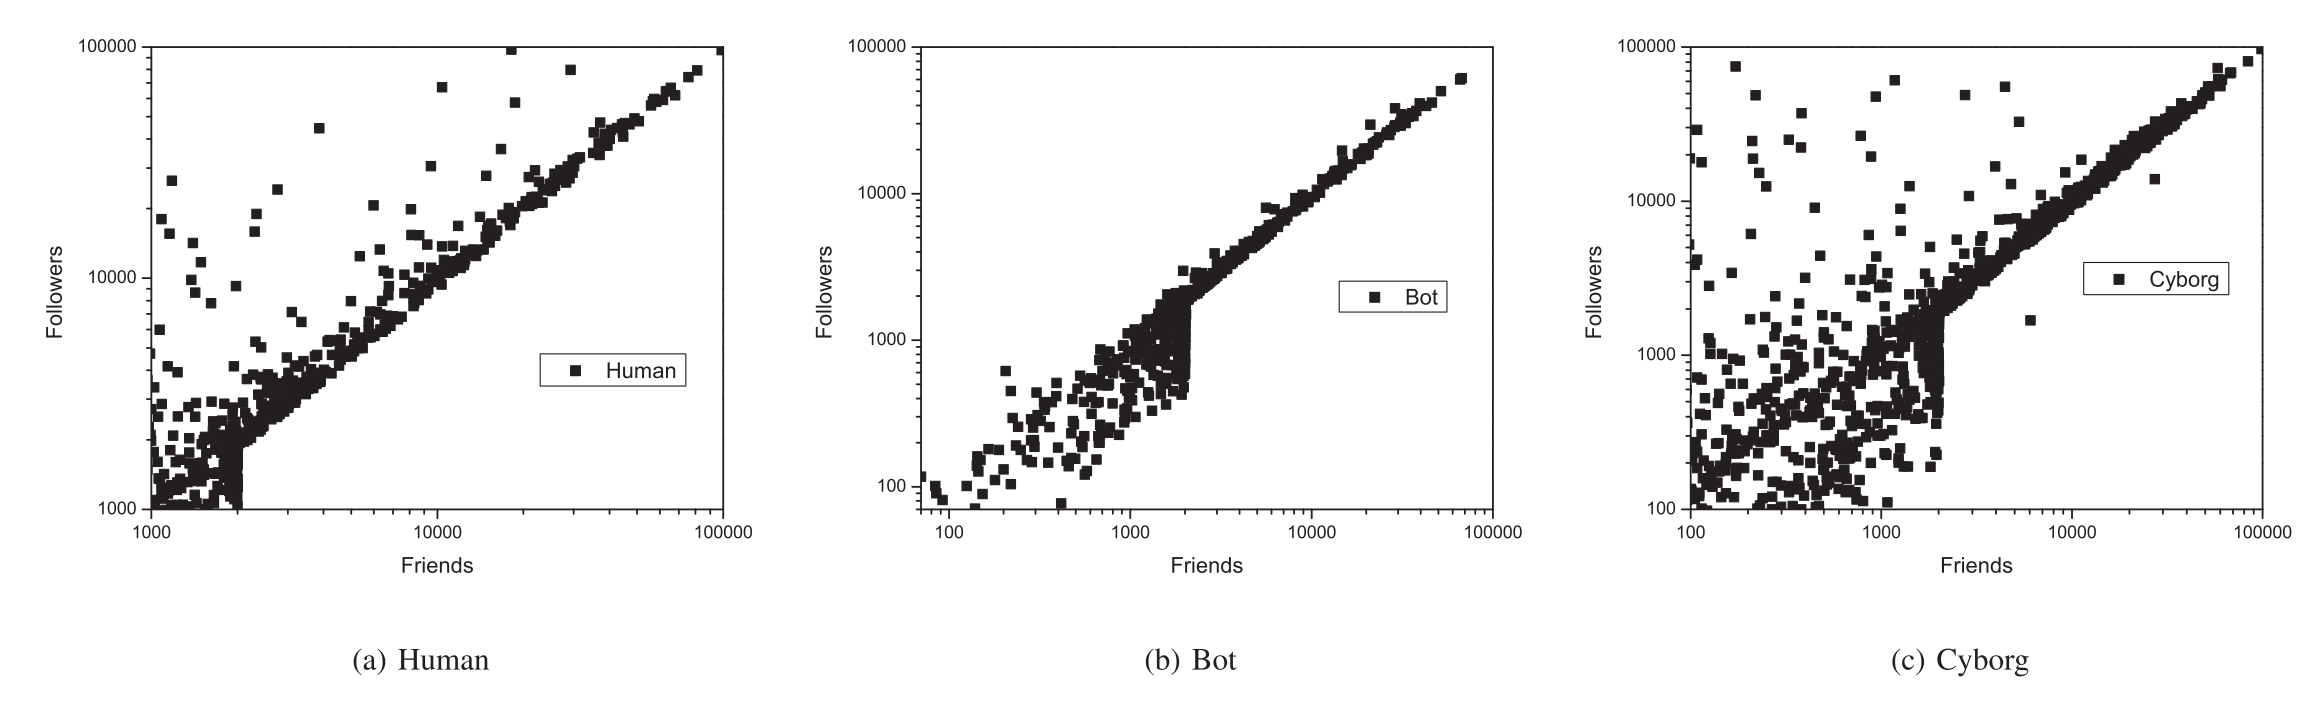
\includegraphics[width=1\textwidth]{template-thesis-latex-master/images/Account_reputation.png}
        	\caption{\textcite[814]{DetectingAutomation} compared the number of friends to the number of followers for human, bot, and cyborg accounts.
        	}
        	\label{figure:humanBotCyborg}
        \end{figure*}
        

        When analysing the number of tweets generated, \textcite[815-818]{DetectingAutomation} found it surprising, that even though bot's tweets are automated, their tweet count is lower than that of humans. This is because, although bots tweet more frequently than humans in their active period, they often take long-term hibernation. In order to compare the regularity of tweeting, the relative entropy was calculated to measure periodic or regular timing of the posting behaviour. This concluded that while bots post tweets at fixed interarrivals (regular behaviour), humans post irregularly (high entropy). When comparing the way tweets are posted, it is evident that humans more commonly post tweets manually via the Twitter website (50.53\%), or also via mobile applications and desktop clients. 42.39\% of the bot-generated tweets were created via unregistered API-based tools, which can be manipulated by bots. Furthermore, it resulted that bots post more external URLs than human users do. As mentioned earlier in this section, bots use URLs to redirect users to external webpages, potentially containing malicious or spam content. When comparing the weekly tweeting behaviour, figure \ref{figure:humanBotCyborgWeekly} shows that humans are more active during the week (workdays, Monday to Friday) than on the weekend. Bots however exhibit approximately the same activity every day. Cyborgs are most active on Monday, then slowly decrease during the week and pick up again on Sunday. Since cyborgs' messages originate from news and blog activities, these tend to be higher at the start of the week, thus explaining the cyborgs' trend.
        
        \begin{figure}[h]
        	\centering
        	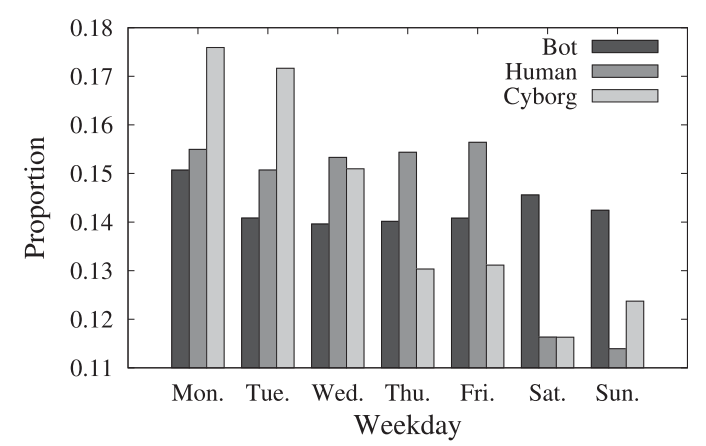
\includegraphics[width=0.5\linewidth]{template-thesis-latex-master/images/weekly_behaviour_tweets.png}
        	\caption{\textcite[818]{DetectingAutomation} analysed the weekly tweet behaviour for humans, bots, and cyborgs.
        	}
        	\label{figure:humanBotCyborgWeekly}
        \end{figure}
        






\subsection{Bot detection systems}

    \subsubsection{DARPA Twitter Bot Detection Challenge}
    \label{subsubsection:DARPA}    
    In 2015 DARPA\footnote{https://www.darpa.mil} (Defense Advanced Research Projects Agency) held a 4-week competition in which six teams competed against each other to identify a set of influence bots on the OSN Twitter. \textcite[39-40]{theDarpaTwitterBotChallenge} introduce and describe the challenge and the methods the top three teams used to detect bots. The competition was called “Twitter Bot Detection Challenge” and the goal for the competing teams was to detect Twitter bots supporting a certain subject. 
    The three winning teams were in unison, as they found that machine learning techniques alone were not suitable to detect the planted bots, due to the lack of training data. What did help, was a semi-automated process including machine learning. Several features were of interest in creating the training set. 
    
    When addressing "Feature-Based Social Bot Detection", \textcite[101]{RiseOfSocialBots} specified that the advantage of examining behavioural patterns, is that the patterns are simple to encode in features and can be adopted with machine learning techniques. One can thereby learn the signature of human-like and bot-like behaviours and classify accounts by observing their behaviours.
    
    \textcite[40-42]{theDarpaTwitterBotChallenge} justified that the feature data that was used in the competition per user was updated periodically. Here are some of the features mentioned by Subrahmanian et al. grouped into categories:
    
    \begin{itemize}
        \item Tweet Syntax: 
            \begin{itemize}
                \item Average number of hashtags, user mentions, links, and special characters used in tweets
                \item Average number of retweets by the user
                \item Percentage of tweets that end with punctuation, a hashtag, or a link (such tweets might be automatically generated)
            \end{itemize}
        \item Tweet Semantics:    
            \begin{itemize}
                \item Number of user posts related to the chosen subject
                \item Most frequent topics that the user tweets about
                \item Number of languages the user’s tweets were generated in (accounts posting tweets in multiple languages may be bots)
            \end{itemize}
        \item Temporal Behavior Features:
            \begin{itemize}
                \item The duration of a user’s longest session without a short break (users that are on Twitter all day without having any breaks are unlikely to be humans)
                \item Average number of tweets per day (if this number is large, the user is more likely a bot)
                \item Percentage of dropped followers. The percentage of “unfollows” compared to the percentage of “follows”. A user who, for example, deleted many followers compared to the number of people he was following could be abnormal (aggressive following behaviour as mentioned in section \ref{subsection:BehaviouralPatternsBotsDisplay}).
            \end{itemize}
        \item User Profile Features:
            \begin{itemize}
                \item Did the user’s profile have a photo? Was that photo taken from a stock image database?
                \item Number of posts/retweets/replies/mentions, followers/followings and sources used by the user such as: mobile applications, desktop browsers, or “null” for missing sources
                \item Similarity of user profile to known bots
            \end{itemize}
        \item Network Features:
            \begin{itemize}
                \item Number of known bots followed by a user (a user following several known bots is more likely to be a bot)
                \item Number/Percentage of bots in a cluster to which a user belonged to (if the user is placed in a cluster with a lot of bots by a clustering algorithm, he or she is more likely to be a bot)
                \item Average clustering coefficient of retweet and mention network associated with each user

            \end{itemize}
    \end{itemize}
    These are just a few of the features per category.
    
    
    
    
    

    \textcite[43]{theDarpaTwitterBotChallenge} list bot analysis algorithms that were used during the competition:
    \begin{itemize}
        \item \textit{Hashtag Co-Occurrence Network:} Unique hashtags are represented by nodes. When two hashtags appear together in a tweet, this is represented by an edge connecting two nodes. These are weighted by the number of times the two hashtags appear together. This algorithm was used to locate other campaign-related hashtags, thus expanding the list of relevant keywords.
        \item \textit{Distance Measurers:} One team detected bots by calculating the cosine similarity between human users and known bots. The results showed, that the distance between two bots is smaller than that of the bot-human pair.
        \item \textit{Online Prediction:} That same team also used a multi-arm bandit based online prediction strategy. This refers to pulling the arms on multiple slot machines to enhance the win, thus learning the probability distribution to which the machines provide a payoff. Every user account received a prediction score between 0 and 1 assigned by each “arm” (classifier). The closer the score was to 1, the more likely the corresponding user account was a bot. Each round, the arm weights are updated and a final “bot score” is produced for every user. This is calculated as a weighted average of the prediction scores of each arm. The account that possessed the highest bot score was then classified as a bot. Through this algorithm, significant classifiers (“arms”) gain weight and insignificant ones gradually lose it.
        \item \textit{Outlier Detection:} The assumption of two teams was that it would be inefficient for bot creators to handmake each bot one by one. They concluded that a number of bots are more likely to be generated by one programme, changing the bot creating algorithm by varying one or more parameters for each of these group of bots. This would mean, that there are similarities between bots created by the same programme. By applying certain detection methods, one team deduced, that bots were outliers.
    \end{itemize}
    
        As stated before, \textcite[40, 44]{theDarpaTwitterBotChallenge} deduced that machine learning on its own would not suffice to detect bots, since different and increasingly sophisticated methods are being used to create bots. They believe detecting bots to be a semi-automated process which builds on four techniques: inconsistency detection and behavioural modelling, text analysis, network analysis, and machine learning. They suggested a three-step workflow combined with strong supporting software to detect bots in an overall detection framework:
        
        \begin{enumerate}
            \item \textit{Initial Bot Detection:} Firstly, identify a few bots. During the competition, in order to expose these first bots, teams used the following four classes of cues:
                \begin{itemize}
                    \item heuristics (e.g. bots whose profile photos were stock images) 
                    \item behaviours (e.g. number of posted tweets over extended periods of time)
                    \item linguistic cues (e.g. tweets with unusual grammar)
                    \item inconsistencies (e.g. the Twitter handle “MaryJones17” with a profile photo of bearded older man)
                \end{itemize}
            \item \textit{Clustering, Outliers, and Network Analysis:} The bots found in step one are valuable, since bots connect to each other to increase follower counts and retweets. As acknowledged earlier in this section, bot developers use programmes to generate bots with varied parameters. Bots that share parameters may create clusters. Clusters of known bots might also contain other bots. This can be exploited to find these other bots.
            \item \textit{Classification/Outlier Analysis:} Standard classifiers (e.g. support vector machines) can be used to detect further bots, once a certain number of humans and bots have been discovered.
        \end{enumerate}
    
    
    
    
    
    
    
    \subsubsection{Botometer (formerly BotOrNot)}
    \label{subsubsection:Botometer}
    \textcite[273-274]{BotOrNotASystem} present a framework in their paper, a socialbot detection system released in May 2014 called BotOrNot (now Botometer). It is a publicly available service that can detect the extent a Twitter account is a bot by analysing features. The authors of this paper (except Clayton A. Davis) were also authors of "The DARPA Twitter Bot Challenge" (\textcite[]{theDarpaTwitterBotChallenge}). In order to evaluate the Twitter account, BotOrNot first needs to collect the account’s history. It uses Twitter’s REST API\footnote{dev.twitter.com/rest/public} to obtain this information. This data is then forwarded to the BotOrNot server. The server calculates how likely the account is a bot using a classification algorithm.
    
    As stated by \textcite[281]{OnlineHumanBotInteractions}, the features are extracted from data and meta-data about social media users, including friends, tweet content and sentiment, network patterns, and activity time series. The collected data is refined into 1150 features grouped into six different classes:
    \begin{itemize}
        \item \textit{User-based features:} e.g. number of friends and followers, the number of tweets produced by the users, profile description and settings
        \item \textit{Friends features:} Varol et al. consider four types of links between Twitter users: retweeting, mentioning, being retweeted, and being mentioned. For the friends features they extract features about language use, local time, popularity, etc.
        \item \textit{Network features:} The Twitter network structure is important when characterising different types of communication. Varol et al.’s network is based on the user’s retweets, mentions and hashtag co-occurrence. Users are nodes in retweet and mention networks. Retweets and mentions are depicted as a directed link between the two users involved. In hashtag co-occurrence networks there are undirected links connecting hashtag nodes. These networks are weighted to the frequency of interactions of co-occurrences. 
        \item \textit{Temporal features:} Temporal features related to user activity are measured. This includes average rates of tweet construction over different time periods and distributions of time intervals between events.
        \item \textit{Content and language features:} The system described in this paper doesn’t capture the quality of tweets. Instead it assembles statistics about length and entropy of tweet text. It also applies the Part-of-Speech (POS) tagging technique to extract language features.
        \item \textit{Sentiment features:} Sentiment analysis describes the emotions conveyed in a text and also the attitude or mood of a whole conversation. The framework uses several sentiment extraction techniques to generate different sentiment features. 
    \end{itemize}

    \textcite[284]{OnlineHumanBotInteractions} trained models using each of the six classes alone, so that they could compare the usefulness of the various features. The user meta-data features led to the best performance, while content features also proved to be effective. When analysing the single features, it turned out that sentiment, content of mentioned tweets, statistical properties of retweet networks, and features of the friends who the user interacts with are valuable.
    
    \textcite[281-282, 284]{OnlineHumanBotInteractions} further explained, that the BotOrNot system was trained using a publicly available dataset of 15K Twitter bots and 16K human accounts. Using the Twitter Search API, the authors collected the most recent tweets created by these accounts. They limited the tweets' collection, thus receiving a dataset of 2.6 million tweets created by verified bots and 3 million created by human users.
    When examining a classifier in a generic evaluation experiment, the classifier is provided with numerical vectors. Every one of these describes the features of an account. A numerical score is returned by the classifier, the higher the score, the more likely the account is a bot. The Random Forest algorithm achieved the best classification performance of 0.95 average AUC (Area Under the receiver operating characteristic Curve) score, when compared to AdaBoost, Logistic Regression and Decision Tree classifiers. This paper measures the quality of splits using the Random Forest model trained using 100 estimators and Gini coefficient.
    Since bots are continuously evolving, the models must constantly be updated based on recent training data. It is also necessary to determine whether the system trained on a dataset’s predictions continues to be reliable and consistent when tested on different data (in the wild).
    When comparing human annotators and machine-learning models, Varol et al. observed that neither performed flawlessly. They discovered that humans’ strengths lie in generalising and learning new features from observed data. Machines are at their strongest when it comes to processing large numbers of relations and searching for complex patterns. 
    
    
    \subsubsection{Other detection systems}
    \textcite[356, 359, 362-363]{AAFA} introduce a new stance detection and bot identification framework called Associative Affinity Factor Analysis (AAFA). The framework distinguishes real people from bots. The proposed model was the first implementation (to the best of the authors knowledge) of Twitter bot detection that uses factor analysis. It begins with creating a latent class profile on Twitter user account metadata. It then also creates the average sentiment score of their tweets. Finally, it implements multiple factor analysis on the mixed feature dataset, which is composed of the metadata and derived attributes.
    The AAFA framework resulted to be highly accurate. When compared to the industry's most popular tool BotOrNot (Botometer), by performing on a Twitter dataset to distinguish bots and humans, the proposed framework achieved 0.96 accuracy, while BotOrNot only achieved 0.66. 
    
    \textcite[630-634]{PreprocessingFrameworkTwitter} approach the socialbot detection on Twitter as a supervised classification problem. After extensive data preprocessing and feature extraction operations, they use machine learning algorithms to detect bots. Their preprocessing framework extracts 62 features, which were inspired by DARPA's Twitter Bot Challenge (described in section \ref{subsubsection:DARPA}), for each user. These were divided into three main groups and after expriments, the most important features for the classification where found: user profile based features (e.g. Number of Followers, Number of Tweets, Has Default Profile Image, etc.), tweet based features (e.g. Maximum Same Hashtag, Most Active Hour, Longest Session Duration, etc.) and periodic features (e.g. Friends Number, Follower Count). The machine learning classifier ultimately uses these features. The authors focused on collecting data from tweets on a trending topic in Turkish. The results led to 86\% accuracy using Gradient Boosted Trees ensemble learning algorithm.
    
    
\section{Conclusion}
\label{sectionb:Conclusion}
The aim of this thesis is to understand and explain what bots are, how they operate, how they can be misused on Online Social Networks (OSNs) and what systems can detect and prevent them. Section \ref{subsection:WeaknessesOSNs} revealed, that in order to prevent bots from infiltrating OSNs, current weaknesses in OSNs would need to be fixed. OSN security defences appear to be more advantageous in detecting bot infiltrations, as opposed to preventing them, which is why this thesis focuses more on detecting bots.
Section \ref{subsection:MisuseOfBots} explains, that various bots can operate differently. This could potentially make them harder to be recognised. However, as discussed in section \ref{subsection:BehaviouralPatternsBotsDisplay}, bots often show specific behavioural patterns when operating on OSNs. Feature-based detection systems, such as Botometer, can exploit these features to detect OSN accounts exhibiting bot like behaviour. OSNs could suspend accounts classified as bots. Twitter's defence mechanisms already suspend suspicious bots, as indicated in section \ref{subsection:BehaviouralPatternsBotsDisplay}. Examples for bot-like behaviour include: messages' lack of intelligence or originality, excessive automatically created content, presence of malicious URLs, aggressive following behaviour, clusters of bots and long online sessions. Feature-based detection is not the only way bots can be detected. The Associative Affinity Factor Analysis (AAFA) achieved higher accuracy than Botometer using factor analysis. The results discovered in section \ref{subsection:WeaknessesOSNs}, stating that only 4.9\% of the users of that study had their account set to protected, suggests that OSN users may not be sufficiently informed about the dangers on OSNs. Section \ref{subsubsection:Botometer} declared that since bots are continuously evolving, the systems must constantly be updated based on recent training data. As stated in section \ref{section:Introduction}, the advances in this area are just beginning and employed strategies are not as advanced as would be liked. The computing community is currently designing advanced methods to detect socialbots automatically. This might lead to improved defence systems in the future. 



 % the main text

%\input{acknowledgements}

\ifmmtpaper

\printbibliography

\else % only use the following for thesis format

\newpage
\printbibliography

\fi


 % group open
\ifmmtpaper 
\begingroup 
    % is required because paper template messes with sizes
    \fontsize{12}{18}\selectfont        
    \setlength{\parindent}{0pt}
    \setlength{\parskip}{5pt plus 2pt minus 1pt}
    \sectionfont{\fontsize{14}{15}\selectfont}
\fi

\newpage
\onecolumn
\begin{appendices}

\section{git-Repository}
Link zum Repository auf dem MMT-git-Server {\url{gitlab.mediacube.at}}:

{\color{red}\url{https://gitlab.mediacube.at/fhs41216/bachelorarbeit-1-troth.git}}
	
\end{appendices}

% group closing
\ifmmtpaper
\endgroup
\fi


\end{document}
